The proposed analytical design integrates voxel-based and non-voxel-based radiomic feature extraction from T1 and T1/T2 images with a \ac{NN} model to predict structural connectivity metrics, including \ac{FA}, \ac{MD}, and relative connectivity values.

\section{Architecture}

The core architecture, as schematically represented in \reflink{fig:model0}{Figure}, consists of two primary components:
\begin{itemize}
\item \textbf{Feature Extraction}: This step involves generating voxel-based and non-voxel-based feature vectors from the T1 and T1/T2 images.
\item \textbf{\ac{FNN}}: A regression or classification head that processes the extracted feature vectors to predict target outputs, such as \ac{FA}, \ac{MD}, or relative connectivity values.
\end{itemize}

\begin{figure}[H]
\centering
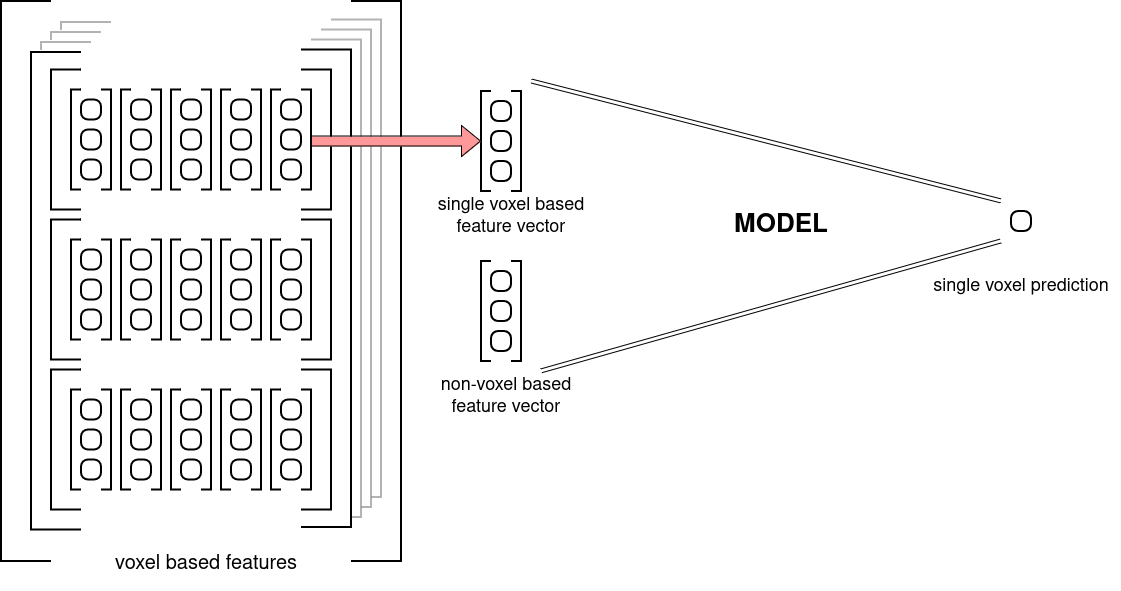
\includegraphics[width=1\textwidth]{model0}
\caption{Architecture Overview}
\label{fig:model0}
\end{figure}

\section{Data Representation}

A crucial distinction exists between volumetric spatial data, such as T1 and T1/T2 images or their corresponding voxel-based features, and individual feature vectors. While the model operates at the feature vector level, lacking global context, certain evaluation processes are performed at the record level.\par
\textbf{This report will refer to the control/patient spatial data as '{\color{red} Record}'} \emph{("voxel based features" in \reflink{fig:model0}{Figure})} \textbf{and to individual feature vectors as '{\color{red} Datapoint}'} \emph{"single voxel based feature vector" and "non-voxel based feature vector" in \reflink{fig:model0}{Figure})}\textbf{.}

\section{Preprocessing}
\label{sec:preproc}

\subsection{Raw Data}
All provided records are in the \ac{NIfTI} format, which need to be parsed. This format stores the raw output of the \ac{MRI} record (an example of which is shown in \reflink{tab:datas1}{Table}), and additionally an affine transformation matrix used for aligning different spaces.

\begin{table}[H]
\begin{adjustwidth}{-.5in}{-.5in}
\centering
\begin{tabular}[H]{|l|l|c|c|l|l|}
\hline
\textbf{Data} & \textbf{Shape} & \textbf{Range} & \textbf{Type} & \textbf{Space} & \textbf{Reference} \\ \hline
\ac{DTI} & (118, 118, 60, 74) & $[0,4096]$ & uint & diffusion & diffusion \\ \hline
Diffusion \ac{FA} & (118, 118, 60) & $[0,1]$ & float & diffusion & diffusion\_fa \\ \hline
Diffusion \ac{MD} & (118, 118, 60) & $[0,0.01]$ & float & diffusion & diffusion\_md \\ \hline
T1 & (208, 256, 256) & $[0,~1000]$ & float & t1 & t1 \\ \hline
T1/T2 & (208, 256, 256) & $[0,1]$ & float & d\_aligned & t1t2 \\ \hline
Cortical Targets & (118, 118, 60, 14) & $\{0,1\}$ & bool & diffusion & targets \\ \hline
Relative Connectivity & (118, 118, 60, 14) & $[0,1]$ & float & diffusion & connectivity \\ \hline
Streamline Image & (118, 118, 60, 14) & $[0,5000]$ & uint & diffusion & streamline \\ \hline
\ac{ROI} Mask (Basal Ganglia) & (118, 118, 60, 2) & $\{0,1\}$ & bool & diffusion & mask\_basal \& roi \\ \hline
Brain Mask & (208, 256, 256) & $\{0,1\}$ & bool & t1 & mask\_brain \\ \hline
Basal Ganglia Segmentation & (208, 256, 256) & $[0, 58]$ & uint & t1 & basal\_seg \\ \hline
\end{tabular}
\end{adjustwidth}
\caption{Raw Data}
\label{tab:datas1}
\end{table}

\subsubsection{Brain Mask}
The provided dataset did not apply the brain masks for the T1 images out of the box so it can be done with a simple element-wise multiplication of the T1 image and T1 mask.

\subsubsection{Registration}
The process of aligning different records into the same native space is called "registration". The provided dataset comes with with 2 (3) different spaces, earlier referenced to as t1 and diffusion (and d\_aligned). Most of the data are in diffusion space, thus it is logical to register the rest into the same space. After manual inspection, only 15 records required registration, out of which only 3 required a tiny translation, while the remaining 12 needed a complete affine registration.\par

The image T1/T2 is the odd one out, as it is inherently in a different space from diffusion (due to them being different resolution), but they are aligned into diffusion space. Although they are practically already registered, this has to be taken into account later on.

\subsubsection{Normalization}
The process of warping each brain into a common space is called "normalization". Applying the \ac{FNIRT} warp fields is more or less straightforward, as two warp fields are provided, one for the diffusion space and one for the T1 space. Note that this process inherently contains the benefits of registration, as it is warping the different images into a common brain shape and space. This also paves the direction of future experiments, as it opens the door to working in either native or normalized space.\par

The only encountered obstacle was with the T1/T2 image. As it is aligned in diffusion space, but \ac{FNIRT} convention ignores the affine transformation of the \ac{NIfTI} format, thus making its registration useless as the raw data of the t1t2 has nothing to do with the raw diffusion data (due to them being different resolution). The solution is to apply an affine matrix to t1t2's raw data which transforms it into t1's raw data space, after which the t1's \ac{FNIRT} warp field can be applied to the t1t2 image. This affine transformation matrix can be easily calculated from the already given matrices. Let $A$ denote T1/T2's affine matrix and $B$ denote T1's affine matrix (after registration), thus the matrix which transforms the T1/T2 into T1 space is $M = A \cdot B^{-1}$.

\subsubsection{Basal Ganglia Segmentation}

As the tractography of the brain is performed on the diffusion image, it inherently means that the connectivity maps and the \ac{ROI} are in diffusion space. But the basal ganglia's subcortical segmentation is in T1 space. This means that even if they are registered in the same space, they will not have a voxel perfect union due to the different resolutions.

\begin{figure}[H]
\centering
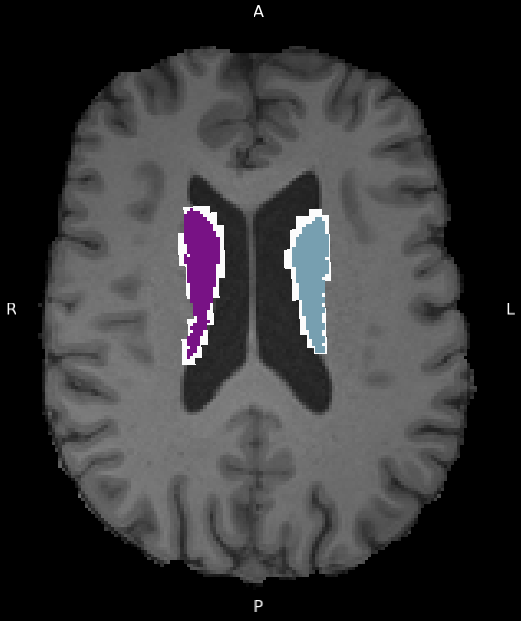
\includegraphics[width=0.3\textwidth]{basal_seg}
\caption{Basal Ganglia Subcortical Segmentation}
\label{fig:basal_seg}
\end{figure}

\reflink{fig:basal_seg}{Figure} visualizes the alignment of the Caudate subcortical region, where the white (larger) region is the Basal Ganglia mask from the diffusion space and the colored (smaller) regions are the Basal Ganglia segmentation from T1 space.\par

In order to keep the data consistent, mapping the segmentation to the Basal Ganglia mask can be done by assigning the same label for each voxel in the basal ganglia as the label of the closest voxel in the subcortical segmentation.

\subsubsection{N-Dim Array}
The used \ac{NIfTI} format stores the raw voxel space and the affine transformation matrix separately, in order to not loose data in the process of interpolating voxels when applying the transformation. But in order to consistently compare voxel data across different spaces (even if they are registered in the same space), the transformation needs to be applied, computing the interpolated voxels in the common space, bringing them into the same raw format of matching X, Y and Z dimensions, and discarding the stored affine matrices.\par

By default, the native anatomical space's origin is near the center of mass of the brain, between the ears. This makes sense for medical professionals, when working with \ac{MRI} records, but data structure-wise an array is indexed from 0, meaning that, after applying the transformation to the voxel space, the yielded array will only contain one quadrant of the record, as the rest are clipped in the negative regions. Thus, the space also needs to be translated with the negative vector of the transformed space's bounding box's lower end.\par

The translation value can be calculated by calculating the boundaries of the transformed space's bounding box. Get all 8 corners of the voxel space and apply the transformation matrix to all of them. Then get the min-max coordinates along X, Y and Z from the 8 transformed vectors, yielding the lower and upper bounds of the transformed space's bounding box.\par

It is very important to use the same translation value across different spaces to properly align them in the native space. For example let $D$ and $T$ denote a diffusion and t1 records and $M_D$ and $M_T$ denote their respective transformation matrices. Let $T_D$ and $T_T$ denote their respective translation values. In order to properly align them we need to apply $A_D = (M_D \cdot {\color{red}T_D})$ matrix and $A_T = (M_T \cdot {\color{red}T_D})$ matrix to $D$ and $T$ respectively, with matching ${\color{red}T_D}$ translation values.\par

The last issue is the missaligned shape of the dimensions of the T1 and diffusion records. This can be simply fixed by truncating the excess along each dimension.

\subsubsection{Uniform Shape}
After aligning the data into the same space per record, it is still very likely that the individual records will not have a uniform shape. This is because, given that they are in native space, some records will contain a smaller volume brain, some will contain a larger, and they will not be the same.\par
Due to the per-voxel based prediction model architecture, this is not a problem, but fixing so that we can use the data in a spatial model like a \ac{FCNN} can be simply solved by adding padding to the records in order to match their shapes.

\subsection{Quality Control}

Having a low count of records means that if there are even just a few outliers, it can heavily affect the end result. Thus all data were manually inspected to make sure they are as clean as possible.

\subsubsection{Mismatched Data}

Looking through the diffusion, diffusion\_fa and diffusion\_md images, 2 records' \ac{FA} and \ac{MD} images were seemingly from completely different patients. Thus the \ac{FA} and \ac{MD} images were omitted for 2 records.

\subsubsection{Garbled Data}

Looking through the subcortical segmentation of the Basal Ganglia revealed that 1 record had a garbled segmentation. Thus, said basal\_seg image was omitted for 1 record.\par
And one record had a garbled T1 \ac{FNIRT} warp field. Said record was entirely omitted from the normalized set of records.

\subsubsection{Missing Data}

Looking through the relative connectivity and streamline images, 3 records were missing these images, said 3 records were completely omitted as these records are effectively missing the labels.\par
Furthermore, the t1t2 images were missing for 10 records, but these were not omitted completely as the t1 images were present for these records, thus experiments only concerning the t1 can have a bit more available data.

\subsection{Radiomics Features}

Extracting the voxel-based radiomic features requires the tuning of two main parameters, namely the bin width and the kernel width. The binning parameter(s) influence how the intensity values of the image are binned, while the kernel size influences the size of the 'sliding window' similar to a convolution.\par
The two approaches for binning are absolute discretization and relative discretization. In the former, a fixed bin width is chosen and in the latter, a fixed number of bins are chosen and the bin width scales in relation to to the min-max voxel values. The absolute discretization consistently provides statistically significantly more reproducible features than the relative discretization. \cite{bin} Relying on this information, the obvious choice to start with is the absolute discretization.\par
The bin width and the kernel width will be tuned in later experiments, and features calculated with different settings will be concatenated and used simultaneously to improve the results. The default values used will be 25 and 5 for the bin and kernel widths, respectively.\par
The types of radiomic features described in \reflink{tab:radf0}{Table} will be used:
\begin{table}[H]
\centering
\begin{tabular}{|l|c|}
\hline
\textbf{Feature Type} & \textbf{Number of Features} \\ \hline
first order & 18 \\ \hline
\ac{GLCM} & 23 \\ \hline
\ac{GLSZM} & 16 \\ \hline
\ac{GLRLM} & 16 \\ \hline
\ac{NGTDM} & 5 \\ \hline
\ac{GLDM} & 14 \\ \hline
3D shape & 17 \\ \hline
\end{tabular}
\caption{Radiomic Feature Types}
\label{tab:radf0}
\end{table}

\subsubsection{Voxel and non-Voxel-Based}
The 92 features shown in \reflink{tab:radf1}{Table} are voxel based calculated. Voxel-based calculation does not make sense for shape features, as it would just describe the shape of the used kernel, which is constant and independent from the input image. However, the additional shape features in \reflink{tab:radf2}{Table} do make sense for the non-voxel based features, as they can be computed for each target region, both hemispheres of the ROI and the entire brain.

\subsection{Coordinates}

One additional input that can be included in the experiments is the coordinates. Although this approach only makes sense in normalized space, where the images from different records are aligned. This theoretically would allow the model to learn certain anatomical markers based on the location of the voxel, adding a type of global context to the input of the model.\par
Furthermore, this approach can be adopted to the native space, by constructing the normalized coordinate map and then 'de-normalizing' them with an inverse \ac{FNIRT} warp field.

\subsection{Data Augmentation}

The only data augmentation that makes sense involves applying small rotation values to the input images in their native space before calculating radiomic features. Applying transformations to the already extracted features is illogical, as interpolating between voxels in feature space is unlikely to yield the same results as computing features after transforming the input images. In summary, any spatial data transformations should be performed upstream. Furthermore, data augmentation only makes sense in native space, as by definition such transformations would make the normalized image pointless.

\subsection{Scaling and Normalization}
\label{sec:norm}

As the extracted features have very different ranges, it makes sense to follow the standard practice of scaling the data to a fixed range. Inspecting the histogram of some of the radiomic features reveals that most of them follow a bell curve with moderate standard deviation, as in the example shown in \reflink{fig:hist_fie}{Figure} (Firstorder Energy).\par

\begin{figure}[H]
\centering
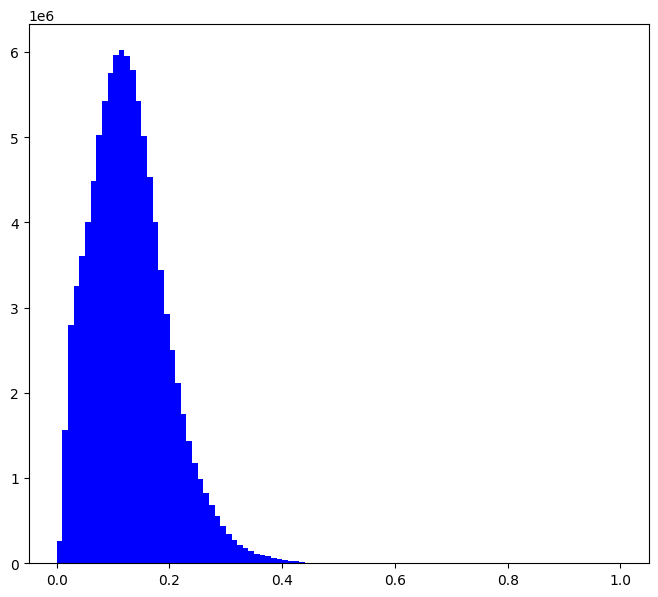
\includegraphics[width=0.4\textwidth]{hist_firstorder_energy}
\caption{Histogram: Firstorder Energy}
\label{fig:hist_fie}
\end{figure}

However, some other features such as those illustrated in \reflink{fig:hist_gls}{Figure} (GLDM Small Dependence High Gray Level Emphasis) and \reflink{fig:hist_ngb}{Figure} (NGTDM Busyness) have a very skewed distribution, the latter one being the most extreme case. This skewing can be mitigated by applying logarithm to the offending features.

\begin{figure}[H]
\centering
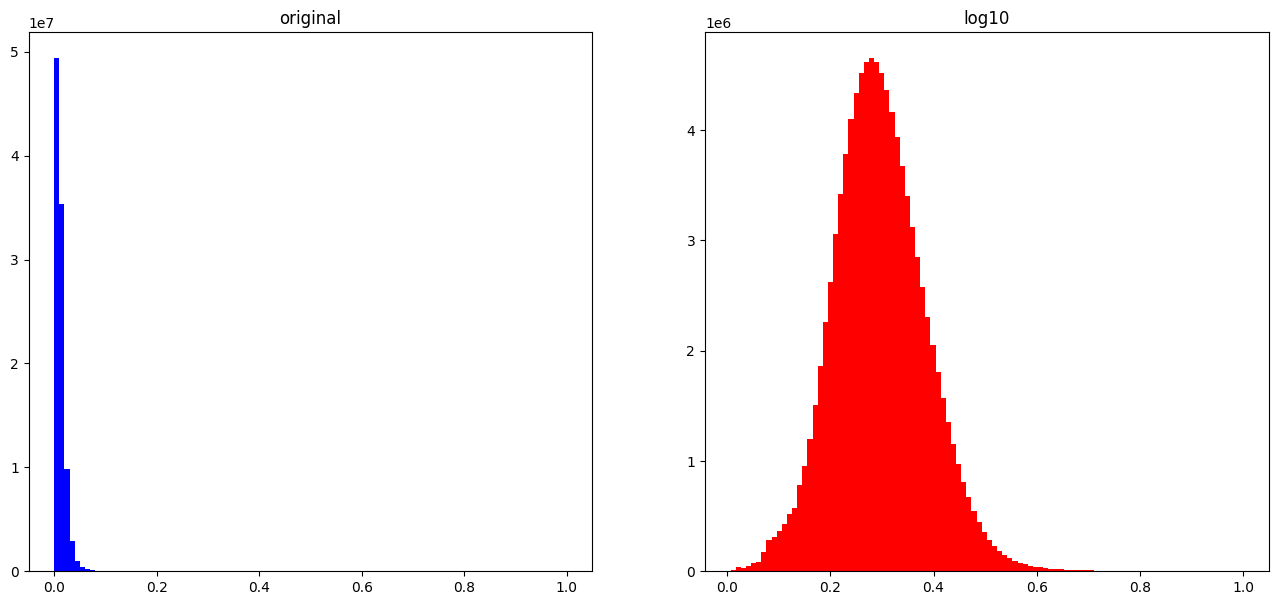
\includegraphics[width=0.8\textwidth]{hist_gldm_small}
\caption{Histogram: GLDM Small Dependence High Gray Level Emphasis}
\label{fig:hist_gls}
\end{figure}

\begin{figure}[H]
\centering
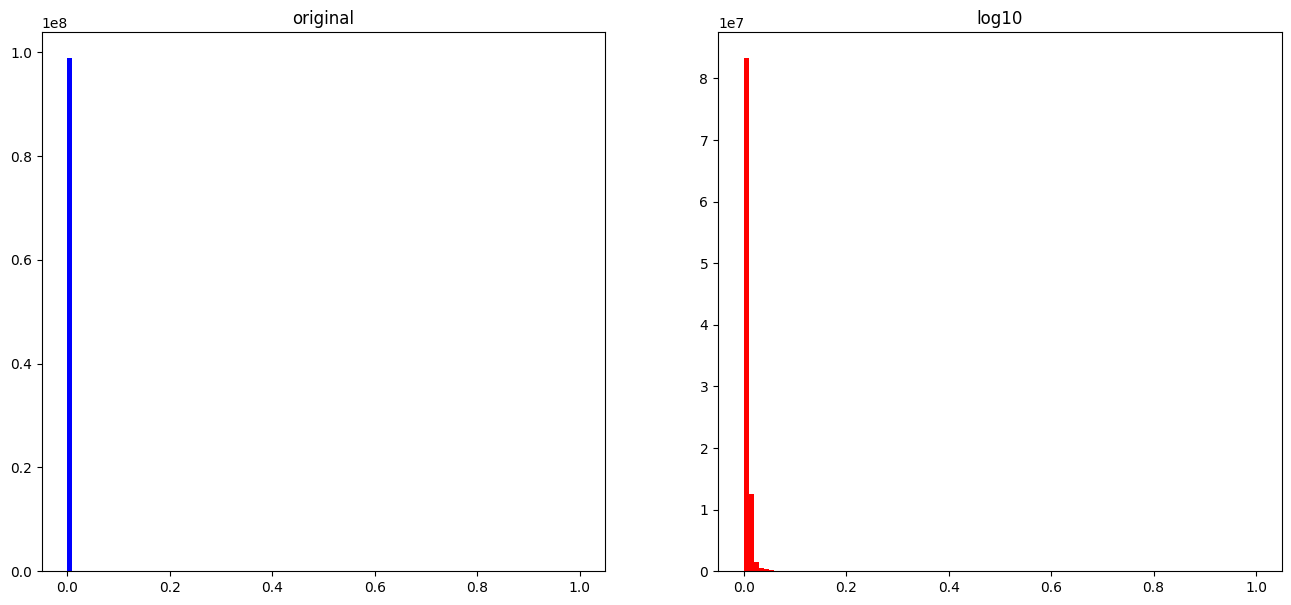
\includegraphics[width=0.8\textwidth]{hist_ngtdm_busyness}
\caption{Histogram: NGTDM Busyness}
\label{fig:hist_ngb}
\end{figure}

Besides the standard benefits of making the optimization process more stable and efficient, and reducing the sensitivity to outliers, this also have some less evident benefits.\par
Although it is very subtle, but storing these records in float16 inherently looses some information. This loss is not a problem for the features that have a healthy distribution, but in the more extreme cases it can cause compression artifacts visible even to the naked eye, such as the very subtle loss of detail in \reflink{fig:gls}{Figure}. And in the most extreme case it can even render the entire feature useless like in \reflink{fig:ngb}{Figure}. While the normalized features have no problem storing this fine detail in float16.\par
This makes the system much more robust from a practical perspective as, depending on the hardware, some GPUs are much more efficient at computing in float16; it also halves the memory and storage requirements as, in float32, a single \ac{MRI} image of 92 volumes (for the 92 features) takes up around 1GB of space.\par
Selecting which features need normalization is done programmatically, and the exact selection criteria is detailed in \reflink{app:imp-norm}{Appendix}.

\subsection{Data Balancing}

Working with highly unbalanced data can be challenging, and fully balancing them does not necessarily help the model's generalization capability. Thus, a method for partially balancing the data will be used, where the bins of the unbalanced data will be up-sampled by a ratio of the difference of the number of datapoints in the bin (compared to the bin with the maximum number of datapoints). Figures \ref{fig:bal_sub} and \ref{fig:bal_con} show how a ratio 1 means perfectly balanced data, 0 means unbalanced data, and how the ratios in between approximately preserve the shape of the distribution and partially balance the data.

\begin{figure}[H]
\centering
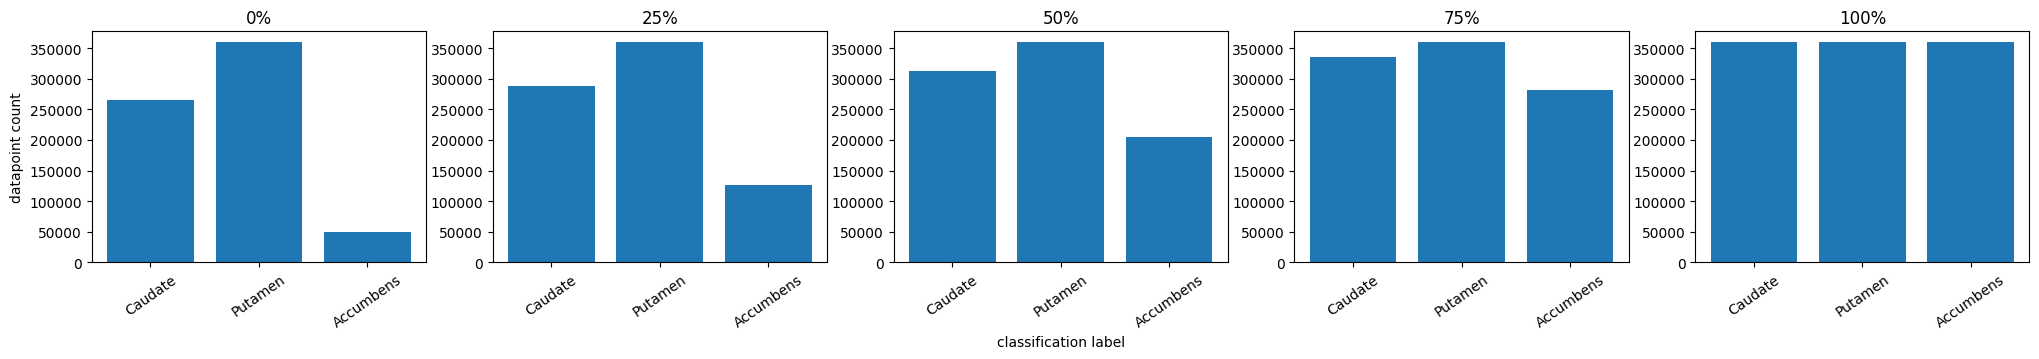
\includegraphics[width=1\textwidth]{bal_subcortical}
\caption{Balance: Subcortical}
\label{fig:bal_sub}
\end{figure}

\begin{figure}[H]
\centering
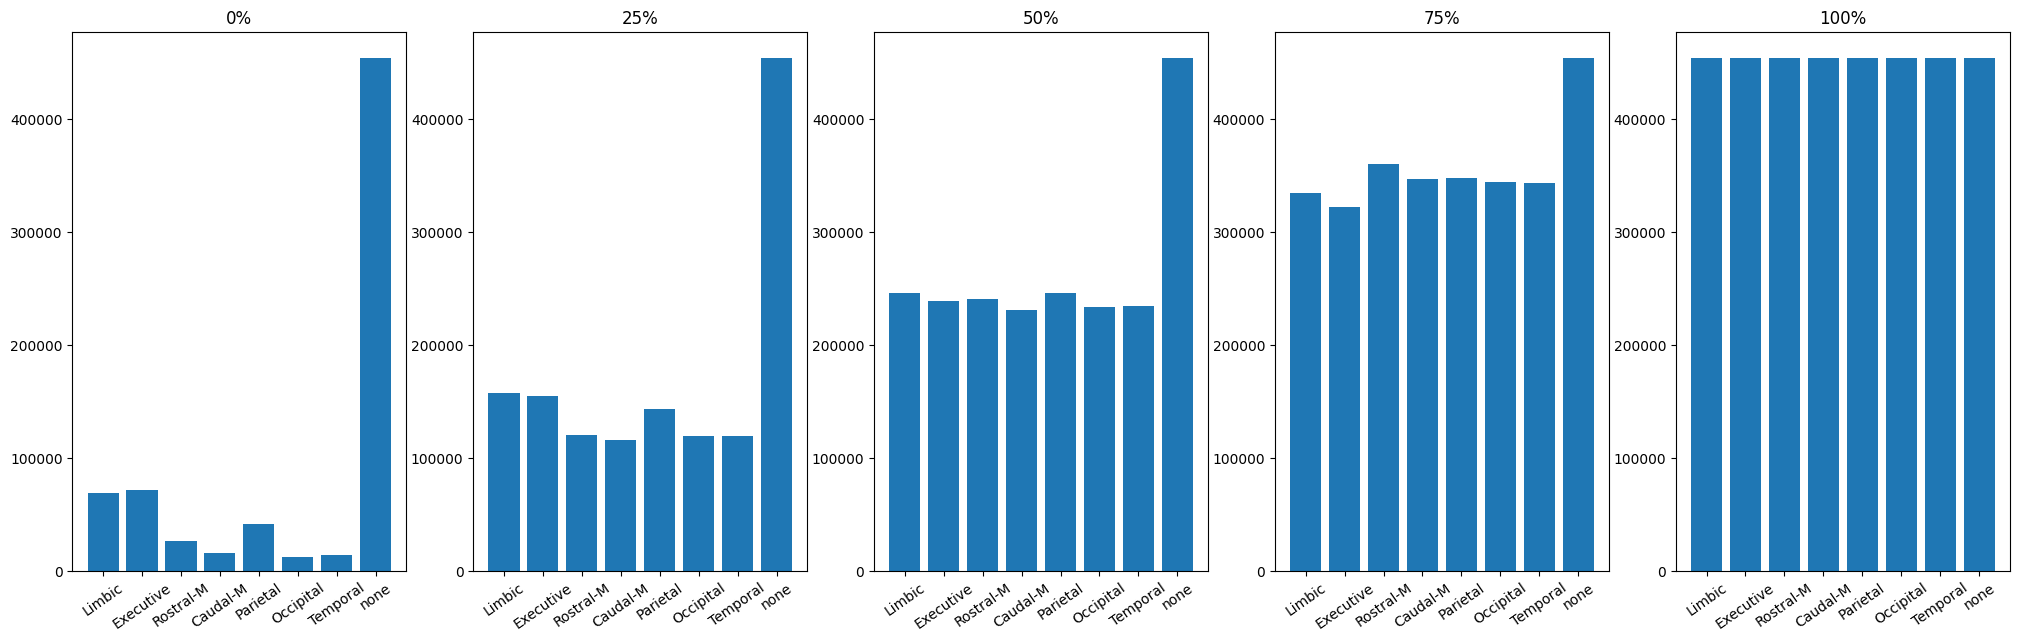
\includegraphics[width=1\textwidth]{bal_connectivity}
\caption{Balance: Relative Connectivity (thresholded at $0.6$ \& binarized)}
\label{fig:bal_con}
\end{figure}

For the diffusion\_md and diffusion\_fa, which are regression problems and have continuous labels, binning can be used to create artificial groups which can be balanced, as illustrated by Figures \ref{fig:bal_md} and \ref{fig:bal_fa}.

\begin{figure}[H]
\centering
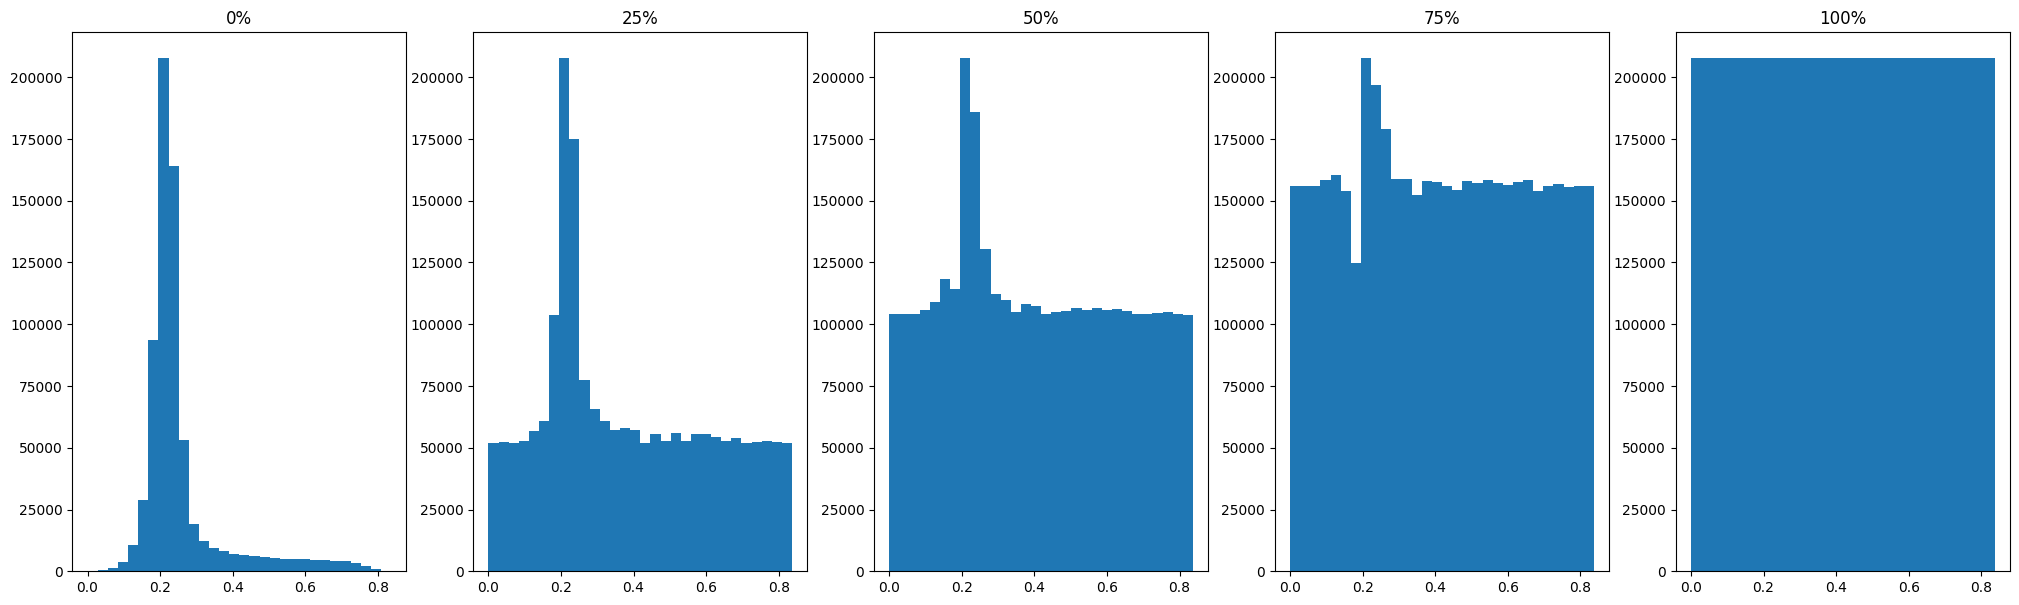
\includegraphics[width=1\textwidth]{bal_diffusionmd}
\caption{Balance: Diffusion MD}
\label{fig:bal_md}
\end{figure}

\begin{figure}[H]
\centering
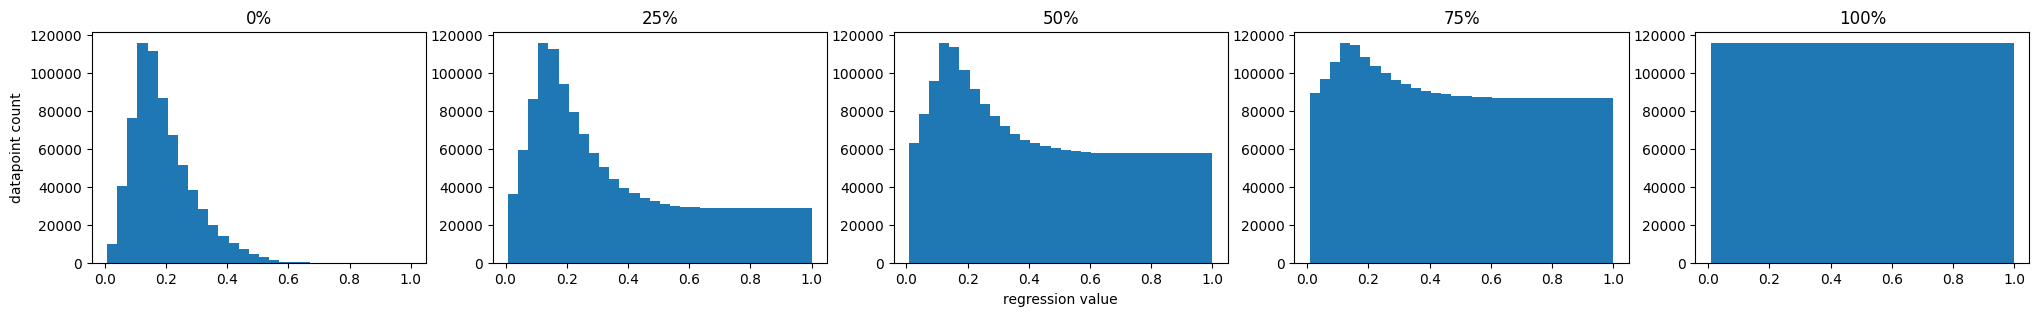
\includegraphics[width=1\textwidth]{bal_diffusionfa}
\caption{Balance: Diffusion FA}
\label{fig:bal_fa}
\end{figure}

\subsection{Clinical Data}
\label{sec:clinical}

There are additional clinical data available for the Patient records. Disease severity can be characterized in terms of \ac{CAP} score, providing a measure of cumulative exposure to the mutant HTT gene \cite{cap}. This widely accepted and used \ac{CAP} score is available for all patients.\par
Another, newer metric for characterizing disease severity is the \ac{cUHDRS} \cite{uhdrs}, which is calculated from 4 other basic metrics: Total Functional Capacity, Total Motor Score, Symbol Digit Modalities Test and Stroop Word Reading. These are available for most patients, with a handful of exceptions.\par
Also, there are a total of 91 available clinical features, with a relatively high level of missing data in some of them. Moreover, there are 8 additional patients available in the clinical data. These can be used to aid the data imputation for the missing values, and can be omitted afterwards, as these have no corresponding \ac{MRI} records.\par
All clinical features were scaled the range of 0-1 with min-max scaling (per feature). And euclidean distance was used for the following imputation process. The imputation strategy itself consisted of 2 steps, first the few missing \ac{cUHDRS} values were imputed from the \ac{CAP} score. And then the remaining features were imputed from the combined \ac{CAP} and \ac{cUHDRS} values.

\subsection{Relative Connectivity}
\label{sec:conpre}

Relative Connectivity describes the ratio of the number of streamlines going into each cortical target. This means that the Streamline record can be converted into Relative Connectivity by simply dividing by the total number of streamlines in each voxel. With the additional inbetween step of filtering some noise, by thresholding the streamlines at 250 (5\% of the total 5000 streamlines), meaning any voxel which has less than 250 streamlines to a target region are set to zero.\par
Then the relative connectivity could be converted into a label, by picking the label of the cortical target to the highest connection per voxel. However this would yield very noisy labels, as these ratios can be quite balanced between the multiple cortical targets, for example voxels with ratios of 0.31/0.29/0.3/0.1. To mitigate this, the relative connectivity can be thresholded at a value higher than 0.5, meaning a label can only be picked for a voxel if at least half of the connections are going to a single target.\par
But this also means that there can be voxels without labels. This can be dealt with introducing an artificial 'Not Connected' label for these voxels.\par
To achieve the best results and filtering, 0.6 was chosen for the thresholding value, as it also filters potential 50-50 situations and only allows labeling strong connections.

\section{Evaluation}

\subsection{Train, Validation and Test Splits}
\label{sec:travaltes}

There are two important aspects to consider when splitting the data into Train/Validation/Test groups. In order to truly validate the model's generalization capability, the split must happen at a record level and not at a datapoint level. This means that our model can only learn from certain records, and it can be validated on records that it has never seen before, not even partially. As a consequence, the split will not follow the defined ratio at a datapoint level, as it could happen that, by pure chance, the train split contained records with larger volumes, resulting in having more datapoints than the validation split.
\begin{figure}[H]
\centering
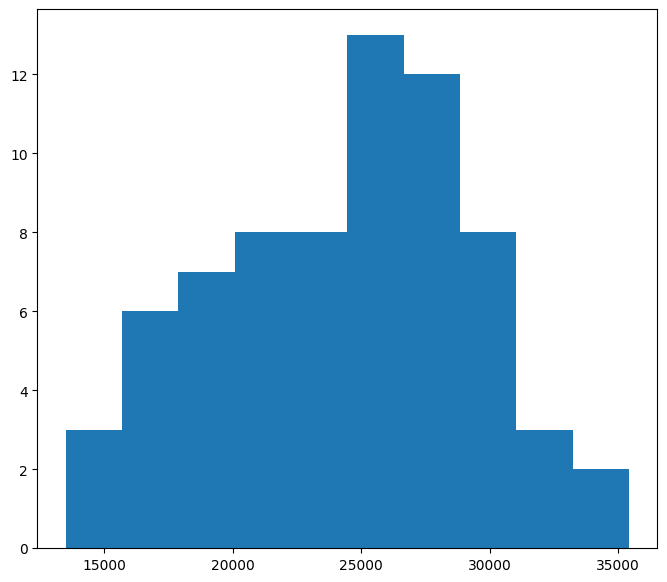
\includegraphics[width=0.5\textwidth]{split}
\caption{Distribution of Records in relation to Datapoints}
\label{fig:hist_split}
\end{figure}
In practice the lower end of datapoint count per record is around half of the higher end. \reflink{fig:hist_split}{Figure} shows the distribution of both Control and Patient records and both Left and Right datapoints. During experimentation, with $0.8$ Train split and $0.5$ Validation/Test split, the datapoint ratios stayed in the range of $0.8\pm0.02$ and $0.5\pm0.06$ for the two split ratios.\par
Furthermore, and to avoid introducing bias in the case of experiments with mixed Control and Patient records, the ratio of Controls/Patients must be kept constant across the different splits. This is required as Controls and Patients can have vast differences due to neurodegeneration. An extra caveat is having another ratio that must also be kept constant for the same reason, which is the symptomatic and asymptomatic patients, as they can also have vast differences due to different stages of neurodegeneration.

\subsection{Accuracy and Pearson Correlation}
\label{sec:eval}

There are three groups of metrics for evaluating each model. First is the 'raw' (will also be referenced as 'train') metric group, which is computed on the datapoints that were extracted with the same hyperparameters as the datapoints during the training process. This means that this metric group best reflects how the model performs on the different splits, such as if the model was trained with a balancing of $0.5$, all splits will be balanced the same way and the metrics will be computed on a datapoint level (the same way as how it is naturally computed in the loss function).\par
The second and third groups are for comparing model performances between models and are for practical evaluation. The difference is that the metrics in this case are computed for each record, and then averaged out between records. This means that they are computed at a record level instead of at a datapoint level, resulting in the elimination of potential bias coming from the deviation from the number of datapoints per records. It also means that these metric groups will inherently ignore data balancing, as it operates on a record level.\par
The second group of metrics is computed in native space, while the third is computed in normalized space. This means that if the model operates in native space, the normalized metrics will be computed by predicting the datapoints for each record, then the spaital record is reconstucted from the datapoints and warped to normalized space, and then the datapoints are extracted from the normalized spatial prediction and compared against the normalized labels (this process would be computationally quite expensive, so the implementation does not follow this exact logic, but it does the same numerically; more information on this in \reflink{app:imp-pre}{Appendix}). This way, the models can have comparable metrics even if they operate in different spaces.











